\documentclass[twosided]{memoir}
\usepackage{mybook}
\usepackage{bigfoot}
\begin{document}
\chapter{Analytic Functions \& Linear Transformations}
\chaptermark{Functions \& Transformations}
\section{Functions}
Let $S$ be a region of the complex $z$-plane. To each point $S$ shall be assigned a number,
\[
w=u+vi
.\] Then $w$ is a \emph{function} of $z$:
\[
	w=f(z)
.\] Instead of a region,$S$, we might have a curve,$C$; or, more generally, any point set $M:\cbr*{z} $ whatever. If to each point $z$ of $M$ a number $w$ is assigned, then $w$ is a function of $z$.

In the case of a real function of a real variable, $y=f(x)$, the function can be represented by a curve, and a real function of two real variables can be represented by a surface. But a complex function $w=u+vi$ of $z=x+yi$ would require a four-dimensional space---the space of the $(u,v,x,y)$. We can, however, represent the function by means of two planes, plotting $z$ in one plane and $w$ in a second plane.

\begin{figure}[htbp]
\centering
\scalebox{0.7}{%
\begin{tikzpicture}
	\draw (0,3)--(0,0)--(3,0);
	\path[draw,use Hobby shortcut, closed=true]
		(0.5,0.5)..(1,1.7)..(1.5,2.4)..(2.4,2.5)..(2,0.4);
	\node at (1,1) {$T$};
	\node[above] at (0,3) {$w$-plane};
	\begin{scope}[xshift=2in]
	\draw (0,3)--(0,0)--(3,0);
	\path[draw,use Hobby shortcut, closed=true]
		(0.5,0.2)..(1,1.5)..(1.5,1.7)..(2,2.3)..(2.4,2.2)..(2.5,0.5)..(0.7,0.4);
	\node[above] at (0,3) {$z$-plane};
	\node at (1,1) {$S$};
	\end{scope} 
\end{tikzpicture}
}
\end{figure}

Thus under suitable conditions a region $S$ of the $z$-plane will be \emph{mapped} on a region $T$ of the $w$-plane. Similarly, a curve $C$ of the $z$-plane will go over into a curve $\Gamma$ of the $w$-plane. Again, if $s_n$ denotes the sum of the first $n$-terms of an infinite series:
\[
u_1+u_2+\dots 
,\] whose terms are complex numbers, then $s_1, \dots $ will be represented by isolated points in the complex plane. 

A point $z=a$ is said to be an \emph{interior} point of a region $S$ if all points within a certain circle about $a$:
\begin{equation}\label{intpoint}
\abs*{z-a} <\delta 
,\end{equation} belong to $S$. By the \emph{neighborhood} of the point $a$ is meant a region having $a$ as an interior point. It may be a region defined by \ref{intpoint}. Or, if
\[
a=\alpha +\beta i, \quad z=x+yi
,\] it may consists of the points $z$ for which
\begin{equation}\label{zdelta}
\abs*{x-\alpha } <\delta , \quad \abs*{y-\beta} <\delta.
\end{equation} In any case, whatever neighborhood be chosen, it is possible to take $\delta $ so that the region \ref{intpoint} or the region \ref{zdelta} lies inside of it. 

Let $M: \, \cbr*{z} $ be any set of points whatever, or a \emph{point set}. By a \emph{cluster point} or \emph{point of condesation}, is meant a point $z=a$ such that there are no points of $M$ distinct from $a$ in every neighborhood of $a$. Thus no matter how small $\delta $ may be chosen, there will be a point $z'$ of $M$ such that
\[
0<\abs*{z'-a} <\delta 
.\] By a \emph{regular arc} is meant the curve:
\[
	x=f(t), \quad y=\phi (t)
,\] where $f(t), \, \phi (t)$ are continuous, together with their first derivatives, in the closed interval $t_0\le t\le t_1$ and $f'(t), \, \phi '(t)$ do not vanish simultaneously. Moreover two distinct values of $t$ shall not yield the same point $(x,y)$.

A \emph{regular curve} is composed of a succession of regular arcs joined at their extremities. It may be open or closed.

The regions $S$ here considered shall be bounded by a finite number of simple regular curves. 

\section{Limits}

Let $M$ be any point set $\cbr*{z} $ having $a$ as a cluster point, and let $f(z)$ be defined in the points of $M$. Then $f(z)$ shall be said to \emph{approach the limit} $b$ when $z$ approaches $a$:
\[
	\lim\limits_{z \to a} f(z)=b
,\] if, to any arbitrary positive number $\epsilon$, there corresponds a positive $\delta $ such that
\begin{equation}\label{limit1}
	\abs*{b-f(z)} <\epsilon,
\end{equation} 
provided that
\[
0<\abs*{z-a} <\delta , \quad z \in M
.\] Geometrically the condition has the following meaning. Let a circle of radius $\epsilon$ be drawn about the point $w=b$ in the $w $-plane, and let a circle of radius $\delta $ be drawn about the point $z=$ in the $z$-plane. Let $z=z'\neq a$ be any point of $M$ lying in the $\delta $-circle, and let
\[
	w'=f(z')
.\] Then $w'$ lies in the $\epsilon$-circle.
\begin{figure}[htbp]
\centering
\scalebox{0.7}{%
\begin{tikzpicture}
	\draw (0,3)--(0,0)--(3,0);
	\node[above] at (0,3) {$v$};
	\node[right] at (3,0) {$u$};
	\draw (1.5,1.5) circle (1);
	\node[below] at (1.5,1.5) {$b$};
	\draw[dashed] (1.5,1.5)--(2.5,1.5);
	\node[above] at (2,1.5) {$\epsilon$};
	\begin{scope}[xshift=2in]
	\draw (0,3)--(0,0)--(3,0);
	\node[above] at (0,3) {$y$};
	\node[right] at (3,0) {$x$};
	\draw (1.5,1.5) circle (1);
	\node[below] at (1.5,1.5) {$a $};
	\draw[dashed] (1.5,1.5) --(2.5,1.5);
	\node[above] at (2,1.5) {$\delta $};
	\end{scope} 
\end{tikzpicture}
}
\end{figure}

\begin{theorem}\label{2.2.1}
A necessary and sufficient condition that $w$ approach $b$ is that
\begin{equation}\label{limit2}
	\lim\limits_{(x,y) \to (\alpha , \beta)} u=U, \quad \lim\limits_{(x,y) \to (\alpha , \beta)} v=V,
\end{equation} 
where
 \[
a=\alpha +\beta i, \quad b=U+Vi
.\] 
\end{theorem} 

\begin{proof}
\begin{enumerate}[i.]
	\item The condition is necessary. Here, by hypothesis, \ref{limit1} is true. Now,
		\[
			w-b=u-U+i(v-V)
		.\] By Chapter 1 Exercise 21,
		\[
		\frac{1}{\sqrt{2} }\sbr*{\abs*{u-U} +\abs*{v-V} } \le \abs*{w-b} 
		.\] Hence
		\[
		\abs*{u-U} < \sqrt{2} \epsilon, \quad \abs*{v-V} <\sqrt{2} \epsilon
	,\] and consequently \ref{limit2} holds. 

\item The condition is sufficient. Here, by hypothesis, \ref{limit2} is true; i.e,
	\[
	\abs*{u-U} <\epsilon, \quad \abs*{v-V} <\epsilon	
	,\] provided
	\[
	\abs*{x-a} <\delta , \quad \abs*{y-\beta} <\delta 
	.\] Hence
	\[
	\abs*{w-b} <2\epsilon
,\] and consequently \ref{limit1} holds. 
\end{enumerate}
\end{proof} 

As a result of \ref{limit1}, we observe that if the limit $b\neq 0$, then there exists a certain neighborhood of the point $a$ such that
\[
	f(z)\neq 0, \quad 0<\abs*{z-a} <h, \quad z \in M
.\] For, choose $\epsilon<\abs*{b} $. Then the point $w=0$ lies outside the $\epsilon$-circle, and we need only set $h$ equal to the $\delta $ corresponding to this $\epsilon$. More generally, let $C$ be any positive number less than $\abs*{b} $:
\[
0<C<\abs*{b} 
.\] Then it is possible to determine $h$ so that
\[
	C<\abs*{f(z)} , \quad 0<\abs*{z-a} <h, \quad z \in M
.\] 
\begin{theorem}
If each of two functions approaches a limit:
\[
	\lim\limits_{z \to a} f(z)=A, \quad \lim\limits_{z \to a} \phi (z)=B
,\] their sum approaches a limit, and the limit of the sum is equal to the sum of the limits:
\[
	\lim\limits_{z \to a} \sbr*{f(z)+\phi (z)} =\lim\limits_{z \to a} f(z)+\lim\limits_{z \to a} \phi (z)
.\] 
\end{theorem} 

\begin{proof}
We wish to show that, to an arbitrary positive $\epsilon$, corresponding to a positive $\delta $ such that
\begin{equation}\label{limsum1}
	\abs*{A+B-f(z)-\phi (z)} <\epsilon,
\end{equation}
provided
\[
0<\abs*{z-a} <\delta , \quad z \in M
.\] By hypothesis,
\begin{align*}
	\abs*{A-f(z)} <\epsilon', \quad 0<\abs*{z-a} <\delta_1, \quad z \in M\\
	\abs*{B-\phi (z)} <\epsilon', \quad 0<\abs*{z-a} <\delta_2, \quad z \in M
\end{align*} where $\epsilon'$ is an arbitrary positive number. Hence by Chapter 1 Exercise 20,
\begin{equation}\label{limsum2}
	\abs*{A+B-f(z)-\phi (z)} <2\epsilon',
\end{equation}
provided
\[
0<\abs*{z-a} <\delta , \quad z \in M,
\] where $\delta $ is the smaller of the two numbers, $\delta_1$ and $\delta_2$. 

Now, $\epsilon$ is the choice of our adversary; but $\epsilon'$ is at our disposal. Let us choose $\epsilon'=\frac{1}{2}\epsilon$. Then \ref{limsum1} follows from \ref{limsum2}, and the proof is complete.
\end{proof} 

\begin{theorem}
If each of two functions approaches a limit:
\[
	\lim\limits_{z \to a} f(z)=A, \quad \lim\limits_{z \to a} \phi (z)=B
,\] their product approaches a limit, and the limit of their product is equal to the product of their limits. 
\end{theorem} 

\begin{proof}
We wish to show that
\begin{equation}\label{limprod1}
	\abs*{AB-f(z)\phi (z)} <\epsilon
\end{equation}
provided
\[
0<\abs*{z-a} <\delta , \quad z \in M
.\] Let
\[
	f(z)=A+\zeta_1, \quad \phi (z)=B+\zeta_2
.\] Then
\begin{align*}
\abs*{\zeta_1} <\epsilon', \quad 0<\abs*{z-a} <\delta_1, \quad z \in M\\
\abs*{\zeta_2} <\epsilon', \quad 0<\abs*{z-a} <\delta_2, \quad z \in M
\end{align*} Now,
\[
	f(z)\phi (z)-AB=B\zeta_1+A\zeta_2+\zeta_1\zeta_2
.\] Hence by Chapter 1 Exercise 20,
\begin{equation}\label{limprod2}
	\abs*{AB-f(z)\phi (z)} \le \epsilon'\abs*{A} +\epsilon'\abs*{B} +\epsilon^{'2}
\end{equation} Choose $\epsilon'$, to begin with, $<1$. Then
\[
\epsilon'\abs*{A} +\epsilon'\abs*{B} +\epsilon^{'2}< \sbr*{\abs*{A} +\abs*{B} +1} \epsilon'
.\] We now choose $\epsilon'$ so that
\[
\sbr*{\abs*{A} +\abs*{B} +1} \epsilon'<\epsilon
\] and take as $\delta $ the smaller of the two numbers, $\delta_1$ and $\delta_2$. Hence \ref{limprod1} follows from \ref{limprod2}, and the theorem is proved.
\end{proof} 

A particular case under the theorem is that in which one of the functions is a constant: $\phi (z)=C$. Thus
\[
	\lim\limits_{z \to a} Cf(z)=C \lim\limits_{z \to a} f(z)
,\] provided $f(z)$ approaches a limit.

\begin{theorem}
If each of the two functions approaches a limit:
\[
	\lim\limits_{z \to a} f(z)=A, \quad \lim\limits_{z \to a} \phi (z)=B
,\] their quotient approaches a limit, and the limit of the quotient is equal to the quotient of their limits:
\[
	\lim\limits_{z \to a} \frac{f(z)}{\phi (z)} =\frac{\lim\limits_{z\to a} f(z)}{\lim\limits_{z\to a} \phi (z)} 
,\] provided 
\[
	\lim\limits_{z\to a} \phi (z)\neq 0
.\] 
\end{theorem} 
\begin{proof}
Begin by choosing $h$ so that
\[
	\frac{1}{2}\abs*{B} <\abs*{\phi (z)} , \quad 0<\abs*{z-a} <h, \quad z \in M
.\] Next, observe that
\[
	\frac{A}{B}-\frac{f(z)}{\phi (z)} =\frac{A}{B}-\frac{A+\zeta_1}{B+\zeta_2} =\frac{A\zeta_2-B\zeta_1}{B\phi (z)} 
\] provided
\[
0<\abs*{z-a} <h,\, \delta_1, \, \delta_2, \quad z \in M
.\] Hence
\begin{equation}\label{limquo1}
	\abs*{\frac{A}{B}-\frac{f(z)}{\phi (z)} } <\frac{\abs*{A} +\abs*{B} }{\frac{1}{2}\abs*{B} ^2} \epsilon'.
\end{equation} and the remainder of the proof presents no difficulty.
\end{proof} 

\emph{The Case that} $z$ \emph{or} $w$ \emph{Becomes Infinite}: If the point set $M : \cbr*{z} $ is not bounded, we say that $f(z)$ \emph{approaches a limit} $b$ when $z$ \emph{becomes infinite}:
\[
	\lim\limits_{z \to \infty} f(z)=b
,\] if to an arbitrary positive $\epsilon$ there corresponds a positive number $G$ such that
\[
	\abs*{b-f(z)} <\epsilon
\] provided
\[
G<\abs*{z} , \quad z \in M
.\] The function $f(z)$ is said to \emph{become infinite} when $z$ approaches $a$:
\[
	\lim\limits_{z \to a} f(z)=\infty
,\] if to an arbitrary large positive number $G$ there corresponds a positive $\delta $ such that
\[
	G<\abs*{f(z)} 
,\] provided 
\[
0<\abs*{z-a} <\delta , \quad z \in M
.\] The definition:
\[
	\lim\limits_{z \to \infty} f(z)=\infty
\] is now obvious. 

A necessary and sufficient condition that
\[
	\lim\limits_{z \to a} f(z)=\infty
\] is that
\[
	\lim\limits_{z\to a} \frac{1}{f(z)}=0
.\] Finally, the fundamental theorem relating to the existence of a limit; \emph{Real Variables}, Chapter II, \S 6 and Chapter III, \S 5; \emph{Funktionentheorie} I, p.30. Stated in the form which corresponds to the positive case it is as follows:

\begin{theorem}[fundamental theorem]
	Let $f(z)$ be defined for all points $z$ which lie outside a certain circle. To an arbitrary positive number $\epsilon$ shall correspond a positive number $M$ such that
	\[
		\abs*{f(z')-f(z'')} <\epsilon, \quad M<\abs*{z'} , \, \abs*{z''} 
	.\] Then $f(z)$ approaches a limit, $U$, as $z$ becomes infinite:
	\[
		\lim\limits_{z\to \infty} f(z)=U
	.\] 
\end{theorem} 
\begin{proof}
Let $\epsilon_1, \epsilon_2, \dots $ be a set of positive numbers such that
\[
\epsilon_1\ge \epsilon_2\ge \dots ; \quad \lim\limits_{n \to \infty} \epsilon_n=0
.\] Let $z_1$ be a point of the region $M_1<\abs*{z} $. Mark the point $w_1=f(z_1)$, and draw a circle of radius $\epsilon_1$ about $w_1$. 
\InsertBoxR{4}{%
\begin{minipage}{0.3\linewidth}
\centering
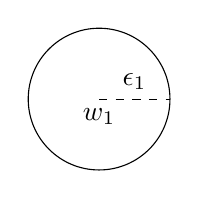
\begin{tikzpicture}[scale=0.6]
	\draw (0,0) circle (1.5);
	\node[below] at (0,0) {$w_1$};
	\draw[dashed] (0,0)--(1.5,0);
	\node[above] at (0.75,0) {$\epsilon_1$};
\end{tikzpicture}
\end{minipage}%
}
\begin{equation}\label{circle1}
\abs*{w-w_1} <\epsilon_1
\end{equation}
Let $M_1, M_2, \dots $ be the values of $M$ which correspond to them by hypothesis, and let $M_1, \le M_2 \le \dots $. Then every point $w=f(z)$, where $M_1<\abs*{z} $, will lie in this circle.

Next, proceed to $\epsilon_2$. Let $z_2$ be a point of the region $M_2<\abs*{z} $. Mark the point
\[
	w_2=f(z_2)
.\] This point lies in the circle \ref{circle1}. Draw a circle of radius $\epsilon_2$ about $w_2$:
\begin{equation}\label{circle2}
\abs*{w-w_2} <\epsilon_2
\end{equation}

\InsertBoxR{3}{%
\begin{minipage}{0.3\linewidth}
\centering
\begin{tikzpicture}[scale=0.7]
	\node at (-0.5,0) {$w_1$};
	\node at (0.65,0) {$w_2$};
	\begin{scope}
		\clip (-0.5, 0) circle (1.5);
	\clip ( 1, 0) circle (1);
	\fill[pattern=north west lines,pattern color=gray!50] (-2,1.5) rectangle (2,-1.5);
	\end{scope} 
	\draw (-0.5,0) circle (1.5);
	\draw (1,0) circle (1);
\end{tikzpicture}
\end{minipage}%
}

Then every point
\[
	w=f(z)
,\] where $M_2<\abs*{z} $, lies in this circle. 

It can happen that the circle \ref{circle2} contains points not included in the circle \ref{circle1}. Such points may be suppressed, since no one of them can represent a value of $f(z)$ when $M_2<\abs*{z} $. Thus only the shaded region is retained.

And now repeat the process, again and again. We thus construct a succession of regions---$S_1$, or the circle \ref{circle1}; $S_2$, the shaded part of the circle \ref{circle2}; and so on---where $S_n$ is bounded by a finite number of arcs of circles, and lies in $S_{n-1} $. Since the maximum diameter of $S_n$ approaches $0$ as $n=\infty$, these regions determine a single point, $U$, which lies within or on the boundary of each, and this is the limit demanded by the theorem. For, if a circle of arbitrarily small radius $\epsilon$ be drawn about $U$, then all the regions $S_n$ from a definite point on, $m\le n$, will lie in the circle, or
\[
	\abs*{f(z)-U} <\epsilon, \quad M_n <  \abs*{z} 
.\] 
\end{proof} 

It is obvious that we might have considered a function $f(z)$ defined merely for a set of points extending to infinity, like the integers $z=1,2, \dots $. The theorem and proof still apply, with the one modification that $z$ must each time be a point of the set. 

Again, instead of a region, or a set of points, extending to infinity, we might have chosen the neighborhood of a finite point $a$, this one point excepted; or we could have let $z$ range over the points of a point set which has $a$ as a point of condensation, not belonging to the set.

\section*{Exercises}

\problem Give the arithmetic details of the proof that the $S_n$ determine a single point, $U$, which lies within or on the boundary of each.
\problem Give all the details of the proof of Theorem \ref{2.2.1}, introducing each time a suitable $\epsilon'$ and showing what $\delta $ is needed and how it is obtained. Illustrate the inequalities geometrically (two sets of figures, each composed of a pair).


\section{Continuity}

Let $f(z)$ be defined in a region $S$ of the $z$-plane. Then $f(z)$ is said to be \emph{continuous in a point} $z=z_0$ of $S$ if
\[
	\lim\limits_{z \to z_0} f(z)=f(z_0)
\] or
\[
	\abs*{f(z)-f(z_0)} <\epsilon,
\] provided
\[
\abs*{z-z_0} <\delta , \quad z \in S
.\] The function is said to be \emph{continous} in $S$ if it is continuous in each point of $S$. 

If $f(z)$ and $\phi (z)$ are two functions, each of which is continuous in a point $z=z_0$, then the functions:
\begin{align*}
&f(z)+\phi (z)\\
&f(z)\phi (z)\\
&\frac{f(z)}{\phi (z)} ,\quad \text{ provided } \phi (z_0)\neq 0
\end{align*}
are continuous in $z=z_0$. 

If $f(z)$ is continuous in $z=z_0$ and does not vanish there, then there is a certain neighborhood of $z_0$:
\begin{equation}\label{zneigh}
\abs*{z-z_0} <h, \quad 0<h,
\end{equation}
throughout which $f(z)$ is different from $0$. Moreover, if
\[
	0<C<\abs*{f(z_0)} 
,\] then $h$ can be so chosen that
\[
	C<\abs*{f(z)} 
\] for all points of the region \ref{zneigh}. 

Let
\begin{align*}
	w&=f(z)\\
	w&=u+vi\\
	z&=x+yi.
\end{align*} A necessary and sufficient condition that $f(z)$ be continuous at the point $z_0$ is, that each of the functions $u$ and $v$ be continuous at the point $(x_0, y_0)$. 

All of these theorems follow at once from the theorems of \S 2. 

\begin{theorem}
A continuous function of a continuous function is a continuous function:
\begin{align*}
	W&=f(w)\\
	w&=\phi (z)\\
	W&=f\pbr*{\phi (z)} 
\end{align*} More precisely, let $f(w)$ be continuous in the neighborhood of a point $w=w_0$ and let $\phi (z)$ be continuous in the point $z=z_0$. Let $w_0=\phi (z_0)$. Then $W=f\pbr*{\phi (z)} $ is continuous in $z=z_0$.
\end{theorem} 

Consider what this theorem means geometrically. If $z$ is a point near $z_0$, then $w=\phi (z)$ will be a point near $w_0$. But when $w$ is near $w_0$, $f(w)$ is near $f(w_0)$. 

Let the student put these considerations into $\epsilon$-form and construct a rigorous proof.

\section*{Exercises}
\problem Show that the function $w=z$ is continuous for all values of $z$. 
\problem Show that the function $w=z^n$ is continuous for all values of $z$, where $n$ is a natural number. 

\problem Show that the function $w=c$ is continuous for all values of $z$. 

\problem Show that a polynomial
\[
	G(z)=a_0z^n+a_1z^{n-1}+\dots +a_n
\] is continuous for all values of $z$. 

\problem Show that a rational function
\[
	R(z)=\frac{f(z)}{\phi (z)} 
\] where $f(z)$ and $\phi (z)$ are polynomials relatively prime, is continuous for all values of $z$ for which it is defined. 

\section{Derivatives}
Let a function
\[
	w=f(z)
\] be defined in a region $S$. Let $z_0$ be an interior point of the region, and let $z_0+\Delta z$ be a second point of $S$. Let
\[
	w_0=f(z_0), \quad w_\Delta w=f(z_0+\Delta z)
.\] Form the difference quotient
\[
	\frac{\Delta w}{\Delta z} =\frac{f(z_0+\Delta z)-f(z_0)}{\Delta z} 
.\] Let $\Delta z$ approach $0$. If the difference quotient approaches a limit, the function is said to have a \emph{derivative} in the point $z_0$. 
\[
	\lim\limits_{\Delta z \to 0} \frac{\Delta w}{\Delta z} =D_zw=f'(z_0)
.\] A necessary condition for a derivative is obtained as follows. Let
\[
w=u+vi, \quad z=x+yi
.\] Since $\Delta w / \Delta z$ by hypothesis approaches a limit as $\Delta z$ approaches $0$, the variable will approach the same limit if $\Delta z$ is restricted to real values, $\Delta z=\Delta x$. Hence
\[
	\lim\limits_{\Delta z \to 0} \frac{\Delta w}{\Delta z} =\lim\limits_{\Delta x \to 0} \pbr*{\frac{\Delta_x u}{\Delta x} +i \frac{\Delta_x v}{\Delta x} } =D_zw
.\] Now,
\[
\lim\limits_{\Delta x \to 0} \frac{\Delta _x u}{\Delta x} = \frac{\partial u}{\partial x} ,\quad \lim\limits_{\Delta x \to 0} \frac{\Delta _xv}{\Delta x} =\frac{\partial v}{\partial x}  
,\] and so
\begin{equation}\label{diff1}
D_zw= \frac{\partial w}{\partial x} =\frac{\partial u}{\partial x} +i \frac{\partial v}{\partial x}.
\end{equation} Similarly, $\Delta z$ may be restricted to values that are pure imaginaries. Thus we find
\[
	\lim\limits_{\Delta y \to 0} \frac{\Delta w}{i\Delta y} =\lim\limits_{\Delta y \to 0} \pbr*{\frac{1}{i}\frac{\Delta _yu}{\Delta y} +\frac{\Delta _yv}{\Delta y} } =D_zw
,\] 
\begin{equation}\label{diff2}
D_zw=\frac{1}{i} \frac{\partial w}{\partial y} = \frac{\partial v}{\partial y} -i \frac{\partial u}{\partial y} 
\end{equation}
Comparing \ref{diff1} and \ref{diff2} we obtain the equations
\begin{equation}\label{creq}
\frac{\partial u}{\partial x} =\frac{\partial v}{\partial y} , \quad \frac{\partial u}{\partial y} =-\frac{\partial v}{\partial x}.
\end{equation}
These are known as the \emph{Cauchy-Riemann Differential Equations}. We have now obtained them as a necessary condition that the function have a derivative. They can be written in the equivalent form
\begin{equation}\label{creq2}
\frac{\partial w}{\partial x} =\frac{1}{i}\frac{\partial w}{\partial y} 
\end{equation}
A very simple function of a complex variable may fail to have a derivative. Consider the function
\[
w=x-yi
.\] Here,
\[
\frac{\partial u}{\partial x} =1, \quad \frac{\partial v}{\partial y} =-1,
\] and the Cauchy-Riemann conditions are not satisfied. It is easy to see directly that this function has no derivative. For
\[
\frac{\Delta w}{\Delta z} =\frac{\Delta x-i\Delta y}{\Delta x+i\Delta y} 
.\] If $\Delta z$ approaches $0$ along the axis of reals, the limit of $\Delta w / \Delta z$ has the value $1$. But if $\Delta z$ approaches $0$ along the axis of pure imaginaries, the limit is $-1$. 

Conversely, let $u$ and $v$ be two real functions defined in the region $S$ and having first partial derivatives satisfying the Cauchy-Riemann Differential Equations. Let these derivatives, furthermore, be continuous. Then the function
\[
	w=u+vi=f(z)
\] will have a derivative, $f'(z)$, and the latter will be continuous in $S$. 
\begin{theorem}
	Let a function $w=f(z)$ where $w=u+vi$ and $z=x+yi$ be defined in a region $S$, and let $u, v$ have continuous first derivatives there. Then a necessary and sufficient condition that $f(z)$ have a continuous derivative is, that the Cauchy-Riemann Differential equations
	\[
	\frac{\partial u}{\partial x} =\frac{\partial v}{\partial y} , \quad \frac{\partial u}{\partial y} =-\frac{\partial v}{\partial x} 
	\] be satisfied. 
\end{theorem} 
\begin{proof}
We have the appraisals
\begin{align*}
	\Delta u&=\frac{\partial u}{\partial x} \Delta x+\frac{\partial u}{\partial y} \Delta y+\zeta_1\Delta x+\zeta_2\Delta y\\
	\Delta v&=\frac{\partial v}{\partial x} \Delta x+\frac{\partial v}{\partial y} \Delta y+\zeta_3\Delta x+\zeta_4 \Delta y
\end{align*} where $\zeta_1, \dots , \zeta_4$ are infinitesimals; i.e. Variables which approach $0$ when $(\Delta x, \Delta y)$ approaches $(0,0)$. On substituting these values into the equation
\[
\frac{\Delta w}{\Delta z} =\frac{\Delta u+i\Delta v}{\Delta x+i\Delta y} 
,\] and reducing, we find, by first-year algebra
\begin{equation}\label{delwz}
	\frac{\Delta w}{\Delta z} =\frac{\partial u}{\partial x} +i \frac{\partial v}{\partial x} +\pbr*{\zeta_1+i\zeta_3} \frac{\Delta x}{\Delta z} +\pbr*{\zeta_2+i\zeta_4} \frac{\Delta y}{\Delta z}.
\end{equation}
Since
\[
\abs*{\frac{\Delta x}{\Delta z} } \le 1, \quad \abs*{\frac{\Delta y}{\Delta z} } \le 1
,\] and since each parenthesis approaches $0$, it is clear that: the right side of \ref{delwz} approaches a limit, when $(\Delta x, \Delta y)$ approaches $(0,0)$, and the value of this limit is given by the first two terms; or
\[
\lim\limits_{\Delta z \to 0} \frac{\Delta w}{\Delta z} =\frac{\partial u}{\partial x} +i \frac{\partial v}{\partial x} 
.\] 
\end{proof} 

\begin{remark}
	If a function $f(z)$ has a derivative at each point of $S$, the derivative is necessarily continuous in $S$ (Goursat's theorem). The proof of this theorem belongs to a later stage in the theory. If, on the other hand, the functions $u$ and $v$ possess first partial derivatives which satisfy the Cauchy-Riemann differential equations, it does not follow that the function $w=u+vi$ is analytic. The derivative and in fact the functions $u$ and $v$ themselves, may fail to be continuous. Consequently some further restriction is required. It is enough, as we have seen, to demand the continuity of the derivatives.
\end{remark} 

\begin{example}
The function $e^z$ has been defined as follows:
\[
	e^{z}=e^x\pbr*{\cos y+i\sin y} 
.\] It has a derivative; for
\[
u=e^x\cos y, \quad v=e^x\sin y
,\] and these functions satisfy the Cauchy-Riemann Differential Equations, since
\[
\frac{\partial u}{\partial x} =e^x\cos y= \frac{\partial v}{\partial y} , \quad \frac{\partial u}{\partial y} =-e^x\sin y= -\frac{\partial v}{\partial x} 
.\] 
\end{example} 

\section*{Exercises}
\problem Let each of the functions $w_1=f(z), \, w_2=\phi (z)$ have a derivative at the point $z=z_0$. Show that the functions $f(z)+\phi (z), \, f(z)\phi (z)$, and $f(z) / \phi (z)$, provided $\phi (z_0)\neq 0$, have a derivative there, and that
\begin{align*}
	&D_z(w_1+w_2)=D_zw_1+D_zw_2\\
	&D_z(w_1w_2)=w_1D_zw_2+w_2D_zw_1\\
	&D_z \frac{w_1}{w_2}=\frac{w_2D_zw_1-w_1D_zw_2}{w_2^2}, \quad \phi (z_0)\neq 0\\
	&D_zF(w)=D_wF(w)D_zw
\end{align*} where $w=\phi (z)$ and $F(w)$ has a derivative in the point $w_0=\phi (z_0)$.

\problem Show that $D_zc=0$ and $D_z z=1$, where $c$ is a constant.

\problem Show that $D_z z^n=nz^{n-1}$, where $n$ is a whole number.

\problem Prove that a polynomial
\[
	G(z)=a_0z^n+\dots +a_n
\] has a derivative.

\problem Show that a rational function has a derivative. 

\problem Let $u, v$ be continuous, together with their first derivatives, in a region $S$, and let them satisfy the Cauchy-Riemann Differential Equations. Let $x=r\cos \phi$ and $y=r\sin \phi$. Show that
\begin{align*}
	\frac{\partial u}{\partial r} &= \frac{1}{r} \frac{\partial v}{\partial \phi } \\
	\frac{1}{r}\frac{\partial u}{\partial \phi } &= - \frac{\partial v}{\partial r} \\
	D_zw&=e^{-\phi i}\frac{\partial w}{\partial r} 
\end{align*}
\problem State and prove the converse of the theorem of the prior exercise.

\problem Show that the function $\log z=\log r+\phi i$, $0\le \phi <2\pi $, has a derivative, and that $D_z\log z=\frac{1}{z}$.

\problem Show that the function $r^x(\cos \alpha \phi +i\sin \alpha \phi )$, $0\le \phi <2\pi $, where $\alpha $ is any real constant, has a derivative.

\problem Let $w=f(z)$ have a continuous derivative in the region $S$. Write $w=R\pbr*{\cos \Theta +i\sin \Theta } $. Show that
\[
	\frac{\partial R}{\partial x} =R \frac{\partial \Theta }{\partial y} , \quad \frac{\partial R}{\partial y} =-R \frac{\partial \Theta }{\partial x} 
,\] and prove the converse.
\problem If in the prior exercise, $z=r(\cos \theta +i\sin \theta )$, show that
\[
\frac{\partial R}{\partial r} =\frac{R}{r}\frac{\partial \Theta}{\partial \theta } , \quad \frac{\partial R}{\partial \theta }=-rR \frac{\partial \Theta}{\partial r}  
,\] and prove the converse.

\section{Differentials}

Let the function $w=f(z)$ have a derivative in the point $z=z_0$:
\[
\lim\limits_{\Delta z \to 0} \frac{\Delta w}{\Delta z} =D_z w
.\] If we set
\begin{equation}\label{infin}
\frac{\Delta w}{\Delta z} =D_zw+\zeta,
\end{equation}
then $\zeta$ is an infinitesimal:
\[
\lim\limits_{\Delta z \to 0} \zeta = 0
.\] From \ref{infin} it follows that
\[
\Delta w=D_zw\Delta z+\zeta \Delta z
.\] Thus the increment $\Delta w$ is broken up into the sum of two infinitesimals:
\begin{enumerate}[i.]
\item $D_zw\Delta z$, a linear function of $\Delta z$,
\item $\zeta \Delta z$, an infinitesimal of higher order.
\end{enumerate} The first term is the \emph{principal part} of the infinitesimal $\Delta w$ and is defined as the \emph{differential} of $w$:
\begin{equation}\label{differential}
dw=D_zw\Delta z.
\end{equation} The differential of the independent variable $z$ is defined as the increment: $dz=\Delta z$. Hence
\begin{equation}\label{increment}
dw=D_zwdz.
\end{equation}
Equation \ref{increment} is true, no matter what the independent variable may be. Suppose that $z$ depends on $t$: $z=\phi (t)$, where $\phi (t)$ has a derivative in the point $t=t_0$, and $z_0=\phi (t_0)$. Then by \S 4, Exercise 1 equation 4,
\begin{equation}\label{Dtw}
D_tw=D_zwD_tz.
\end{equation}
By definition, $t$ now being the independent variable,
\[
dw=D_tw\Delta t, \quad dz=D_t z\Delta t
.\] Hence \ref{increment} follows from \ref{Dtw}. 

\emph{Derivative Along a Curve}: A function $f(z)$ may be defined merely along a curve
 \[
	 x=\phi (t), \quad y=\psi (t)
 ,\] where $\phi (t)$ and $\psi(t)$ are continuous, together with their first derivatives, throughout a closed interval $t_0\le t\le t_1$, and furthermore
 \[
	 0<\phi '(t)^2+\psi'(t)^2
 .\] Thus $w=f(z)=u+vi$ becomes a complex function of the real variable $t$:
 \[
	 w=F(t)+i\Phi (t)
 .\] $w$ is said to have a \emph{derivative} along $C$ if $\Delta w / \Delta t$ approaches a limit:
 \[
 \lim\limits_{\Delta t \to 0} \frac{\Delta w}{\Delta t} =D_tw
 .\] A necessary and sufficient condition is, that $F(t)$ and $\Phi(t)$ both have derivatives. Then,
 \begin{equation}\label{Dphi}
	 D_tw=F'(t)+i\Phi'(t).
 \end{equation} The differential of $w$ is defined by the equation:
 \begin{equation}
	 dw=D_twdt=F'(t)dt+i\Phi'(t)dt.
 \end{equation}

\section{Analytic Functions}
Let $f(z)$ be defined throughout a region $S$ of the complex $z$-plane, and let $f(z)$ have a derivative, $f'(z)$ at each interior point of $S$. Let $f'(z)$ be continuous\footnote{It can be shown that $f'(z)$ is necessarily continuous in $S$; this is \emph{Goursat's Theorem; Funktionentheorie}, I, p.368. But this is a question which belongs to a later stage of the theory, and so we introduce the hypothesis of continuity at this point.} in $S$. Then $f(z)$ is defined as \emph{analytic} in $S$. 

A function is defined as \emph{analytic in a point} if it is analytic throughout a region which includes the point in its interior. 

The term \emph{holomorphic} is also used, meaning the same thing as analytic in a region.

\section*{Exercises}
\problem Show that the sum, difference, product, and quotient (provided the denominator does not vanish) of two analytic functions is an analytic function. 

Take each of these four theorems by itself. State precisely the hypothesis, and the conclusion. And give a \emph{proof}. 
\problem An analytic function of an analytic function is an analytic function.

State this theorem in detail, and prove it.

\section{The Inverse Function}
Let
\[
	w=f(z)
\] be analytic in the point $z=z_0$, and let $f'(z_0)\neq 0$. Each point $z$ of the neighborhood of $z_0$ is carried over into a point $w $ of the neighborhood of $w_0$. And now I say: \emph{If the neighborhood of $z_0$ is suitably restricted, the map of this region on a portion of the $w$-plane will be one-to-one, and consist of a region $T$ of the latter plane}. 

The proof of this theorem follows at once from the theorems relating to Implicit Functions and the Inverse of a Transformation, \emph{Real Variables}, Chapter IV, \S 12. It is here a question of the inverse of the transformation:
\[
	u=\phi (x,y), \quad v=\Psi(x,y)
,\] where $z=x+yi$ and $w=u+vi$. 

The functions $\phi (x,y)$ and $\Psi(x,y)$ are continuous, together with their first partial derivatives, in the neighborhood of the point $(x_0,y_0)$, and it remains merely to examine the Jacobian:
\begin{equation}\label{jacob}
	J=\frac{\partial (u,v)}{\partial (x,y)} =\frac{\partial u}{\partial x} \frac{\partial v}{\partial y} -\frac{\partial u}{\partial y} \frac{\partial v}{\partial x}.
\end{equation}
Now, because of the Cauchy-Riemann relations
\[
\frac{\partial u}{\partial x} =\frac{\partial v}{\partial y} , \quad \frac{\partial u}{\partial y} =-\frac{\partial v}{\partial x}
,\] we have
\[
	J=\pbr*{\frac{\partial u}{\partial x} } ^2+\pbr*{\frac{\partial v}{\partial x} } ^2
.\] Hence
\[
	J|_{z=z_0} =\abs*{f'(z_0)} ^2\neq 0
,\] and so all the conditions of the theorem are fulfilled. It follows, then, that the transformation defined my $w=f(z)$ is equivalent to a transformation $z=F(w)$, where $F(w)$ is single-valued and continuous throughout a certain region $T$ of the $w$-plane, including the point $w=w_0$ in its interior.

Let us formulate the result as a theorem, and supplement it by the face that the inverse function is also analytic.

\begin{theorem}\label{realvarthm}
	Let $f(z)$ be analytic throughout a circle $K$:
	\[
	\abs*{z-z_0} <h
,\] and let $f'(z_0)\neq 0$. Then it is possible, on suitably restricting $h$, to find a circle $H$:
\[
	\abs*{w-w_0} <h', \quad w_0=f(z_0)
,\] such that the equation $w=f(z)$, where $w$ is an arbitrary point of $H$, admits one and only one root $z$ in $K$. The function $z=F(w)$ thus defined is analytic in the point $w=w_0$.
\end{theorem} 
To prove that $F(w)$ has a derivative, form the difference quotient
\[
	\frac{\Delta z}{\Delta w} =\frac{F(w_0+\Delta w)-F(w_0)}{\Delta w} 
.\] Since $\Delta z\neq 0$ when $\Delta w\neq 0$, it follows that
\[
	\frac{F(w_0+\Delta w)-F(w_0)}{\Delta w} =\pbr*{\frac{\Delta w}{\Delta z} } ^{-1}
.\] When $\Delta w$ approaches $0$, $\Delta z$ also approaches $0$, and hence the right hand side approaches a limit, namely $(D_zw)^{-1}$. Moreover, $f'(z)$ vanishes nowhere in $K$, if $h$ is suitably restricted, and thus the proof applies to every point of $H$. Hence
\[
D_wz=\frac{1}{D_zw}
.\] The right hand side is a continuous function of $z$, and hence of $w$. This completes the proof.\footnote{It might seem as if this theorem should admit a much more elementary proof, especially if we add to our knowledge the fact that the angle between two curves is preserved, \S 9. The point set $K$ is carried over into a certain region point set $\mathfrak{S}$, and, at least when $h$ is suitably restricted, it is not obvious that $\mathfrak{S}$ must fill out smoothly a certain neighborhood of $w_0$? There are two questions that have to be met: i. Why should $\mathfrak{S}$ cover every part of the neighborhood of $w_0$? In other words, may there not be open spaces---lakes, lacunae---near $w_0$, whose points correspond to no points of $K$? ii. May not $\mathfrak{S}$ overlap itself? In other words, may not a point of $\mathfrak{S}$ correspond to two or more different points of $K?$ 

There seems to be no simpler answers to these questions, than the one given by the Theorem of Implicit Functions---and, indeed, we are fortunate to have so simple an answer as this.}

\section*{Exercises}
\problem In the theorem cited from the \emph{Real Variables} (\ref{realvarthm}) the regions about the points $(x_0,y_0)$ and $(u_0,v_0)$ are rectangles. Explain the transition to circles.
\problem Prove the existence of a derivative of $F(w)$ by means of the Cauchy-Riemann Differential Equations. 
\problem If $y=f(x)$ is a real function of the real variable $x$, where $a<x<b$; and if $f(x)$ has a continuous derivative which does not vanish: $f'(x)\neq 0$, the inverse function is single-valued. 

By analogy in the complex case, let $f(z)$ be analytic in a region $S$ --- say, inside a circle; and let $f'(z)\neq 0$ there. Should you expect the inverse function to be single-valued? Why?


\section{The Transformation $w=az$}

Let the complex $z$-plane be transformed on the $w$-plane by means of the transformation
\begin{equation}\label{w=az}
w=az,
\end{equation}
where $a\neq 0$ is a constant such that
\[
	a=\mathcal{A}e^{zi}=\mathcal{A}\pbr*{\cos \alpha +i\sin \alpha } 
.\] Write $z$ and $w$ in polar form:
\[
	z=r\pbr*{\cos \phi +i\sin \phi } , \quad w=R\pbr*{\cos \Psi+i\sin \Psi} 
.\] Then \ref{w=az} becomes
\begin{equation}\label{Rephi}
	Re^{\Psi i}=\mathcal{A}r e ^{(\phi +\alpha )i}.
\end{equation}
Hence
\begin{equation}\label{R=Ar}
	R=\mathcal{A}r, \quad \Psi=\phi +\alpha.
\end{equation}
Consider, first, two particular cases. The general case can then be compounded out of these. 

\begin{enumerate}
	\item[i.] $\mathcal{A}=1$, $\alpha \neq 0$. Here,
		\[
		R=r, \quad \Psi=\phi +\alpha 
		.\]
\end{enumerate}
Each point $z$ goes over into a point $w$ at the same distance from the origin, but with its angle increased by $\alpha $. Thus the whole plane is rotated about the origin through an angle $\alpha $, without any deformation whatever. It is easier to think of the $z$-plane as \emph{transformed into itself}, rather than on a separate $w$-plane; cf, the first figure.

\begin{figure}[htbp]
\centering
\scalebox{0.7}{%
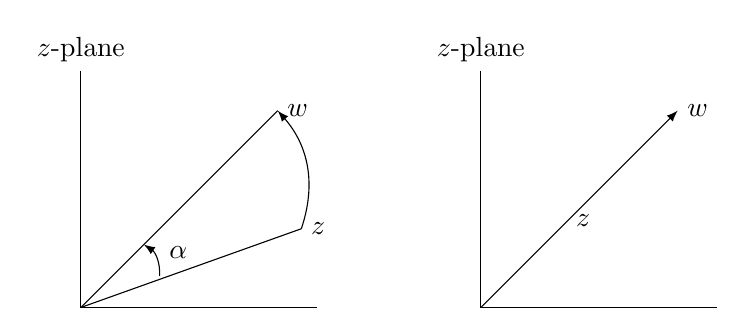
\begin{tikzpicture}
	\draw (0,3)--(0,0)--(3,0);
	\node[above] at (0,3) {$z$-plane};
	\draw (0,0)--(2.5,2.5);
	\node[right] at (2.5,2.5) {$w$};
	\draw (0,0)--(2.8,1);
	\node[right] at (2.8,1) {$z$};
	\draw[bend right, -latex] (1,0.4) to (0.8,0.8);
	\node[below right] at (1,0.9) {$\alpha $};
	\draw[bend right, -latex] (2.8,1) to (2.5,2.5);
	\begin{scope}[xshift=2in]
	\draw (0,3)--(0,0)--(3,0);
	\node[above] at (0,3) {$z$-plane};
	\draw[-latex] (0,0)--(2.5,2.5);
	\node[right] at (2.5,2.5) {$w$};
	\node[below] at (1.3,1.3) {$z$};
	\end{scope} 
\end{tikzpicture}
}
\end{figure}


\begin{enumerate}
	\item[ii.] $\alpha =0$. Here,
		\[
			R=\mathcal{A}, \quad \Psi=\varphi
		.\] 
\end{enumerate} 


A point $z\neq 0$ is moved along the ray drawn from the origin through the point, and it comes to a point $w$ whose distance from $O$ bears to the distance of $z$ from $O$ the fixed ratio $\mathcal{A}$. If $\mathcal{A}>1$, $w$ is further from $O$ than $z$ was. If $\mathcal{A}<1$, $w$ is nearer. 

It is easy to visualize the transformation of the plane as a whole. It is as if it were a rubber membrane, which is stretched equally in all directions, if $\mathcal{A}>1$. If $\mathcal{A}<1$, the membrane is allowed to contract. In this case, the plane is no longer transformed as a rigid body. It is deformed. Nevertheless, figures go over into \emph{similar} figures---a square goes over into a square; a circle into a circle, etc. But the size is changed, always in the linear ratio of $\mathcal{A}:1$. 

The general case represented by \ref{R=Ar} can now be compounded out of these two particular cases. Thus we see that the $z$-plane is rotated through an angle $\alpha $ and stretched in the ratio of $\mathcal{A}: 1$. The order can be reversed --- first, the stretching, then the rotation. 

Transformations play a \emph{most important role} in all branches of mathematics, physics, and geometry, and the student can not begin too early to train himself in this domain of thought. He will do well to turn to the general case of projective transformations, even though these will not concern him in this course; cf. Osgood and Graustein, \emph{Plane and Solid Analytic Geometry}, Chap. XV and Chap. XXIII, \S 10; also \emph{Advanced Calculus}, p. 279, \S 11. 

\section{Preservation of Angles}
Turning now to the general case of an analytic function:
\begin{equation}\label{9.1}
	w=f(z),
\end{equation}
let $f(z)$ be analytic in the point $z=z_0$, and let $f'(z_0)\neq 0$. We have seen that the neighborhood of the point $z_0$ is mapped on the neighborhood of the point $w=w_0$ in a one-to-one manner and continuously. We will now show that two curves, $C_1$ and $C_2$, intersecting at $z_0$ under the angle $\alpha $, go over into curves $\Gamma_1$ and $\Gamma_2$ intersecting at $w_0$ under an equal angle. Since the same is true of any other point $z'$ near $z_0$, the transformation defined by \ref{9.1} is called \emph{isogonal} (\emph{winkeltreu}, having the same angles).

\begin{figure}[htbp]
\centering
\scalebox{0.7}{%
\begin{tikzpicture}
	\draw (0,3)--(0,0)--(3,0);
	\node[above] at (0,3) {$w$-plane};
	\node[right] at (2,1) {$w_0$};
	\draw[bend right] (2,1) to (1,2);
	\node[below] at (1,2) {$\Gamma_2$};
	\draw[bend right] (2,1) to (1.5,3);
	\node[right] at (1.5,3) {$\Gamma_1$};
	\draw[bend right,-latex] (2.1,1.8) to (1.6,1.7);
	\begin{scope}[xshift=2in]
	\draw (0,3)--(0,0)--(3,0);
	\node[above] at (0,3) {$z$-plane};
	\node[below] at (1,1) {$z_0$};
	\draw[bend left] (1,1) to (2.5,1);
	\node[below] at (2.5,1) {$C_1$};
	\draw[bend left] (1,1) to (2.5,2.5);
	\node[right] at (2.5,2.5) {$C_2$};
	\draw[bend right,-latex] (1.6,1.2) to (1.3,1.7);
	\end{scope} 
\end{tikzpicture}
}
\end{figure}
Let $z'=z_0+\Delta z$ be any second point, and let $w'=w_0+\Delta w$ be its image. Since
\[
\lim\limits_{\Delta z \to 0} \frac{\Delta w}{\Delta z} =D_zw
,\] where
\[
	D_zw=A=\mathcal{A}e^{\alpha  i}, \quad \mathcal{A}\neq 0
,\] it follows that
\[
\frac{\Delta w}{\Delta z} =A+\zeta
,\] where $z$ is an infinitesimal such that $\lim\limits_{\Delta z \to 0} \zeta = 0$. Hence
\begin{equation}\label{delw}
	\Delta w=\Delta z\pbr*{A+\zeta}.
\end{equation}
This last equation tells the story. It shows that the angle of $\Delta w$ is nearly equal to the angle of $\Delta z$ plus the angle of $A$:
\[
	\Arc \Delta w=\Arc \Delta z+\Arc\pbr*{A+\zeta} 
.\] Let a curve $C$ be drawn from $z_0$, and let $\Gamma$ be its image. Let $z'$ be a nearby point of $C$, and $w'$ its image. Then the angle that the secant $z_0$, $z'$ makes with the axis of reals, represents $\Arc \Delta z$; and similarly in the $w$-plane. Let $z'$ approach $z_0$. Then
\begin{equation}\label{limarc}
	\lim \Arc \Delta w=\lim \Arc \Delta z+\lim \Arc \pbr*{A+\zeta},
\end{equation}
where $\Phi=\phi+\alpha $.


Equation \ref{limarc} means that, no matter what curve $C$ be drawn from $z_0$, the angle which its tangent makes with the positive axis of reals, plus the constant angle $\alpha $, will give the angle which the tangent to its image, $\Gamma$, makes with the positive axis of reals in the $w$-plane. From this result the isogonal property mentioned at the beginning follows immediately. 

\section{Conformal Mapping}
The isogonal property thrown light on the map defined by the function $w=f(z)$. 

\begin{figure}[htbp]
\centering
\scalebox{0.7}{%
\begin{tikzpicture}
	\draw (0,3)--(0,0)--(3,0);
	\node[above] at (0,3) {$w$-plane};
	\draw (1,2.5) -- (3,0.5);
	\node[below] at (3,0.5) {$w_0$};
	\draw (1,2.5) -- (1.5,1);
	\draw(1.5,1) -- (3, 0.5);
	\fill[pattern=north east lines,pattern color=gray!50] (1,2.5)--(3,0.5)--(1.5,1)--cycle;
	\begin{scope}[xshift=2in]
	\draw (0,3)--(0,0)--(3,0);
	\node[above] at (0,3) {$z$-plane};
	\draw (1,1)--(2,2.5);
	\draw (2,2.5)--(2.7,2.1);
	\draw (2.7,2.1)--(1,1);
	\node[left] at (1,1) {$z_0$};
	\fill[pattern=north west lines, pattern color=gray!50] (1,1)--(2,2.5)--(2.7,2.1)--(1,1)--cycle;
	\end{scope} 
\end{tikzpicture}
}
\end{figure}
Consider a small scalene triangle drawn in the neighborhood of $z_0$. It goes over into a curvilinear triangle into the $w$-plane, which has the same angles. Since the curved sides of the latter triangle look almost like straight lines, the triangle will have the appearance of an ordinary right-line triangle, similar to the first, but magnified in the ratio $\mathcal{A}:1$ and rotated through the angle $\alpha $. And what has just been said of small triangles is true of any small figures, for the figure in the $z$-plane can be covered by a network of small triangles. The smaller the figure, the less relative departure of the image from precise similarity. Because of this property the transformation is called \emph{conformal} (preserving form).

\emph{Element of Arc}: Let the curve $C$ of \S 9 be represented in the usual manner by the equations:
\[
	x=\phi (t), \quad y=\psi(t),
\] where
\[
	0<\phi '(t)^2+\psi'(t)^2,
\] and let the arc be denoted by $s$. The length of the chord is $\abs*{\Delta z} $ and hence
\[
\lim\limits_{\Delta t \to 0} \frac{\abs*{\Delta z} }{\Delta t} =\pm D_ts
.\] Let $S$ denote the arc of $\Gamma$. Then
\[
\lim\limits_{\Delta t \to 0} \frac{\abs*{\Delta w} }{\Delta t} =\pm D_t S
.\] From \ref{delw} it follows that
\[
\lim\limits_{\Delta t \to 0} \frac{\abs*{\Delta w} }{\Delta t} =\lim\limits_{\Delta t \to 0} \frac{\abs*{\Delta z} }{\Delta t} \lim\limits_{\Delta t \to 0} \abs*{A+\zeta} 
,\] and hence
\begin{equation}\label{Dts}
D_tS=D_ts \abs*{D_z w} 
.\end{equation} $\abs*{D_zw} $ is a positive real function of the two real variables $x, y$. Denote it by $M$. Then \ref{Dts} can be written in the form:
\[
dS=M ds
.\] This equation is characteristic of a conformal transformation, and can, indeed, be taken as the definition of such a transformation. 

For a detailed discussion cf. \emph{Funktionentheorie} I, Chap. VI, \S 8, p. 245, and also Chap. II, \S 7, p.74.

Mercator's map of the world affords a simple and interesting illustration from Cartography; cf. \emph{Advanced Caculus}, p. 169. Stereographic projection will be taken up in the next Chapter, \S 6, and may well be studied at this point.

\section*{Exercises}
\problem Study the conformal map by means of the two real equations:
\[
	u=f(x,y), \quad v=\phi (x,y)
\] where $f(x,y), \phi (x,y)$ are continuous, together with their first partial derivatives, and
\[
\frac{\partial u}{\partial x} =\frac{\partial v}{\partial y} , \quad \frac{\partial u}{\partial y} =-\frac{\partial v}{\partial x} 
,\] some of these derivatives being different from zero. 

This is all done in the \emph{Funktionentheorie} I, Chap. II, \S 7, but the student is warned against making a minute study of that treatment. He may give it a cursory glance when he is sleepy. Then, when he is fully mobilized, he should produce it independently. But it is better to defer this exercise till the next chapter has been completed, and then come back to this study.




\end{document}
